\documentclass[titlepage,11pt]{article}
\usepackage{comment}
\usepackage{enumitem}
\usepackage{transparent} % Untuk transparansi gambar
\usepackage{listings}
\usepackage{amsmath}
\usepackage{graphicx}
\usepackage[font=small,labelfont=bf]{caption}
\usepackage[bahasa]{babel}
\usepackage{float}
\usepackage{verbatim}
\usepackage{graphicx,tabularx,multirow}
\usepackage{xcolor}
\usepackage[onehalfspacing]{setspace}
\usepackage[
	allcolors=visigrey,
	colorlinks=true,
]{hyperref}
\usepackage[a4paper,left=2cm,right=2cm]{geometry}
% Pengaturan kutipan artikel
\usepackage[style=ieee, backend=biber]{biblatex}
%Code listing style pak akok
\definecolor{codegreen}{rgb}{0,0.6,0}
\definecolor{codegray}{rgb}{0.5,0.5,0.5}
\definecolor{codepurple}{rgb}{0.58,0,0.82}
\definecolor{backcolour}{rgb}{0.95,0.95,0.92}

\usepackage{eso-pic} % Untuk menambahkan elemen ke seluruh halaman

\newcommand\BackgroundPic{
  \put(0,0){
    \parbox[b][\paperheight]{\paperwidth}{
      \vfill
      \centering
      \transparent{0.1}
      \includegraphics[width=0.4\paperwidth,keepaspectratio]{miot.png}
      \vfill
    }
  }
}

\newcommand\BackgroundAllPages{ \AddToShipoutPicture*{\BackgroundPic} }
\newcommand\BackgroundNone{ \ClearShipoutPicture } % hilangkan background

\lstdefinestyle{mystyle}{
	backgroundcolor=\color{backcolour}, commentstyle=\color{codegreen},
	keywordstyle=\color{magenta},
	numberstyle=\small\color{codegray},
	stringstyle=\color{codepurple},
	basicstyle=\ttfamily\footnotesize,
	breakatwhitespace=false,         
	breaklines=true,                 
	captionpos=t,                    
	keepspaces=true,                 
	numbers=left,                    
	numbersep=5pt,                  
	showspaces=false,                
	showstringspaces=false,
	showtabs=false,           
	frame = single,
	tabsize=2
}
\lstset{style=mystyle}

\definecolor{visigrey}{rgb}{.1,.15,.15}
\geometry{top=1cm,bottom=.5cm}
\savegeometry{titlepage}
\geometry{top=2cm,bottom=2cm}
\savegeometry{main}

\def\bspace{\(\qquad\qquad\qquad\)}
\usepackage[T1]{fontenc}
\usepackage[utf8]{inputenc}
\usepackage{tgheros}
\renewcommand*\familydefault{\sfdefault}

\setcounter{tocdepth}{6}

\def\autor{Laboratorium }
\def\lab{Multimedia dan Internet of Things}
\def\departemen{Departemen Teknik Komputer}
\def\institut{Institut Teknologi Sepuluh Nopember}
\def\praktikum{Laporan Sementara \\ Praktikum Jaringan Komputer}
\def\nama{Abraham Napitupulu - 5024231048}
% Ubah Judul sesuai dengan modul
\def\judul{Firewall \& NAT}
\def\tanggal{2025}
\begin{document}
% Ubah Bahasa sesuai dengan keinginan
\selectlanguage{bahasa}

\BackgroundNone
\def\headingtype{\bf \small}
\loadgeometry{titlepage}

\begin{titlepage}
	\centering
	\begin{tabularx}{\textwidth}{l@{\hskip 0pt}lX}
		\raisebox{-0.5\height}{
\includegraphics[width=3cm]{Cover/img/logodepart.png}} 
		& \raisebox{-0.5\height}{\includegraphics[width=3cm]{Cover/img/miot.png}} 
		& \raggedleft
	\hfill
	\begin{minipage}{0.5\textwidth}
		\raggedleft
		{\emph{\headingtype \autor}} \\[-2pt]
		{\headingtype \lab} \\[-2pt]
		{\headingtype \departemen} \\[-2pt]
		{\headingtype \emph{\institut}}
	\end{minipage}

	\vspace{5cm}
	\end{tabularx}
	
	\vspace{5cm}
	{\Huge \bf \praktikum \par}
	
	\vspace{2cm}
	{\LARGE \bf \judul \par}
	
	\vspace{2cm}
	{\Large \nama \par}
	
	\vfill
	{\Large \tanggal \par}
	
	\vfill
	
\includegraphics[width=\textwidth]{Cover/img/footer.png}
\end{titlepage}

\loadgeometry{main}


\BackgroundAllPages
% Pilih Modul yang akan di build
\section*{Laporan Hasil Percobaan Firewall \& NAT}
\addcontentsline{toc}{section}{Laporan Hasil Percobaan Firewall \& NAT}

\section{Langkah-Langkah Percobaan}
Pada praktikum ini, dilakukan serangkaian konfigurasi pada router MikroTik untuk mengimplementasikan fungsionalitas Network Address Translation (NAT) dan Firewall. Proses ini bertujuan untuk menyediakan konektivitas internet ke jaringan lokal sekaligus mengamankannya dengan aturan filter tertentu.

\subsection*{$\bullet$ Konfigurasi Awal Router}
\addcontentsline{toc}{subsection}{Konfigurasi Awal Router}
Langkah pertama adalah memastikan router berada dalam kondisi konfigurasi default kosong untuk menghindari konflik pengaturan.

\begin{enumerate}
    \item \textbf{Reset Konfigurasi Router:} Perangkat router direset ke pengaturan awal melalui aplikasi Winbox.
    \begin{enumerate}
        \item Akses menu \textit{System -> Reset Configuration}.
        \item Aktifkan opsi \textbf{No Default Configuration} dengan mencentangnya.
        \item Klik tombol \textit{Reset Configuration} untuk memulai proses.
    \end{enumerate}
    \begin{figure}[H]
        \centering
        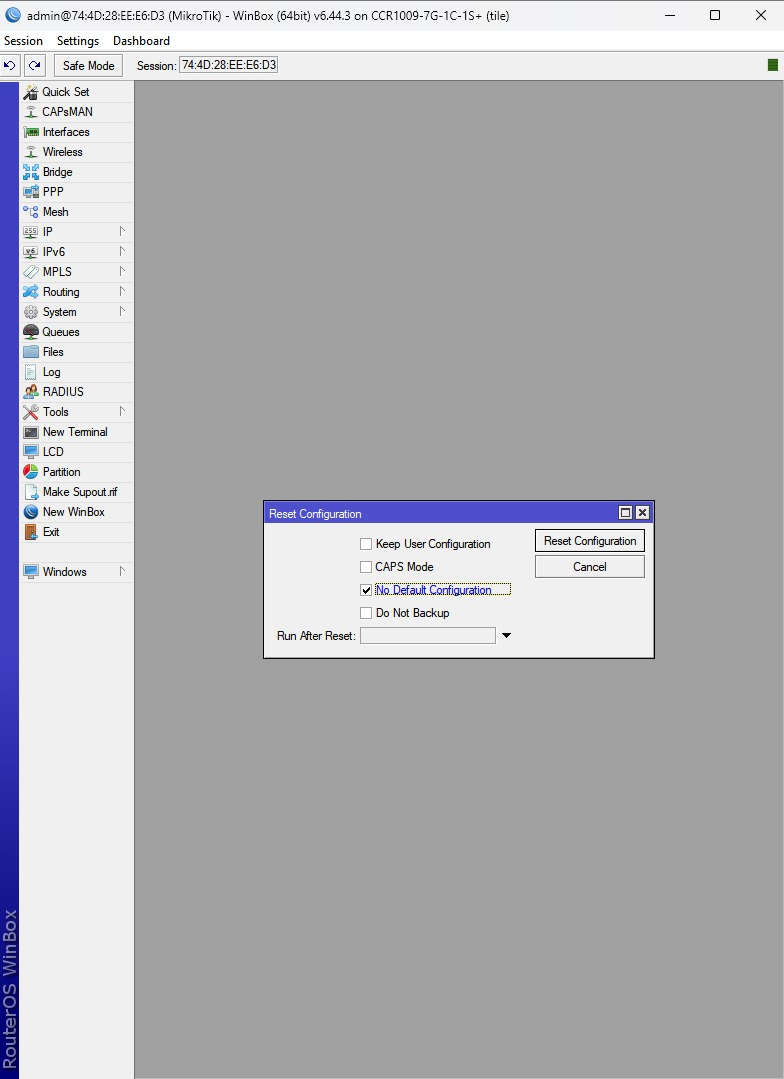
\includegraphics[width=0.6\textwidth]{img4/ResetConfig.jpeg}
        \caption{Pengaturan reset router dengan opsi "No Default Configuration"}
    \end{figure}
    
    \item \textbf{Login ke Router:} Setelah router selesai melakukan reset dan restart, dilakukan proses login kembali menggunakan Winbox dengan MAC address.
    \begin{enumerate}
        \item Username yang digunakan adalah \texttt{admin}.
        \item Kata sandi dikosongkan.
    \end{enumerate}
\end{enumerate}

\subsection*{$\bullet$ Konfigurasi Jaringan dan NAT}
\addcontentsline{toc}{subsection}{Konfigurasi Jaringan dan NAT}
Tahap ini meliputi pengaturan koneksi ke internet (WAN) dan distribusi IP ke jaringan lokal (LAN), serta konfigurasi NAT.

\begin{enumerate}
    \item \textbf{Konfigurasi DHCP Client (ether1):} Antarmuka \texttt{ether1} dikonfigurasi untuk menerima alamat IP secara dinamis dari sumber internet.
    \begin{enumerate}
        \item Akses menu \textit{IP -> DHCP Client}, lalu klik ikon `+`.
        \item Pilih \textit{Interface}: \texttt{ether1}.
        \item Klik \textit{Apply} dan pastikan status menunjukkan \textbf{bound}.
    \end{enumerate}
    \begin{figure}[H]
        \centering
        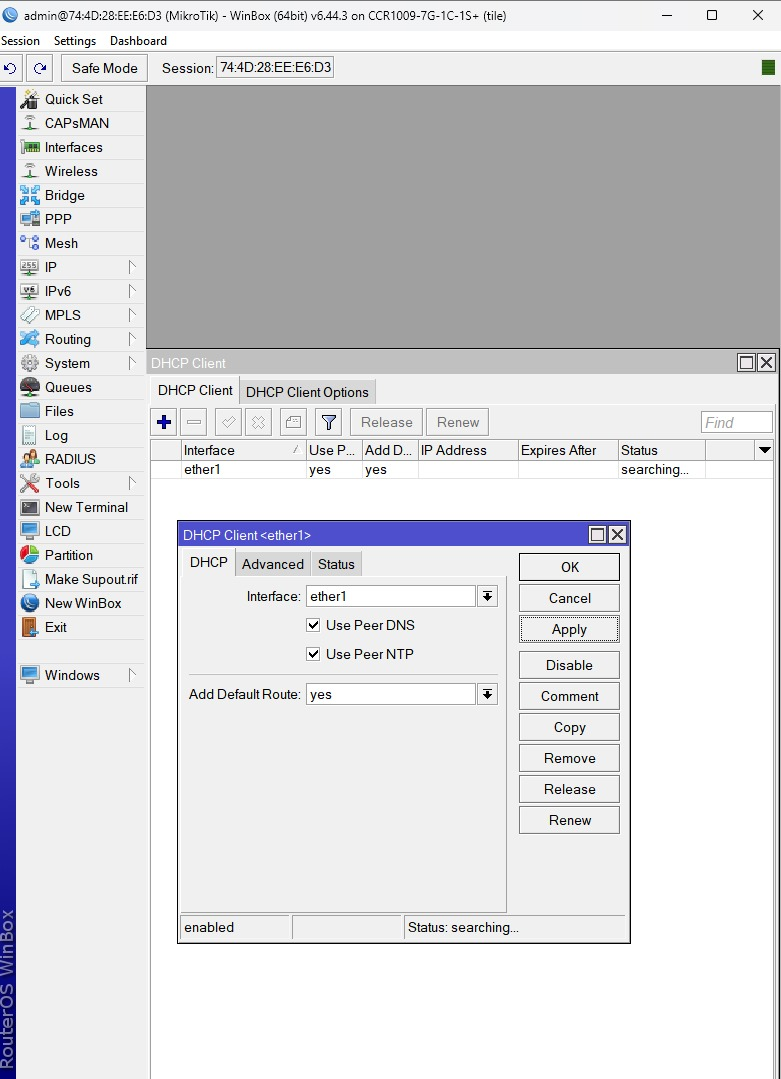
\includegraphics[width=0.7\textwidth]{img4/DHCPCLient.jpeg}
        \caption{Status DHCP Client menunjukkan "bound" setelah konfigurasi}
    \end{figure}
    
    \item \textbf{Penambahan Alamat IP LAN (ether7):} Alamat IP statis ditambahkan ke antarmuka \texttt{ether7} yang akan terhubung ke jaringan lokal.
    \begin{enumerate}
        \item Akses menu \textit{IP -> Addresses}, lalu klik ikon `+`.
        \item Masukkan \textit{Address}: \texttt{192.168.10.1/24}.
        \item Pilih \textit{Interface}: \texttt{ether7}.
    \end{enumerate}
    
    \item \textbf{Konfigurasi DHCP Server:} Router diatur untuk mendistribusikan alamat IP secara otomatis ke perangkat klien di jaringan lokal melalui \texttt{ether7}. Proses ini dilakukan melalui wizard \textit{DHCP Setup}.
    \begin{figure}[H]
        \centering
        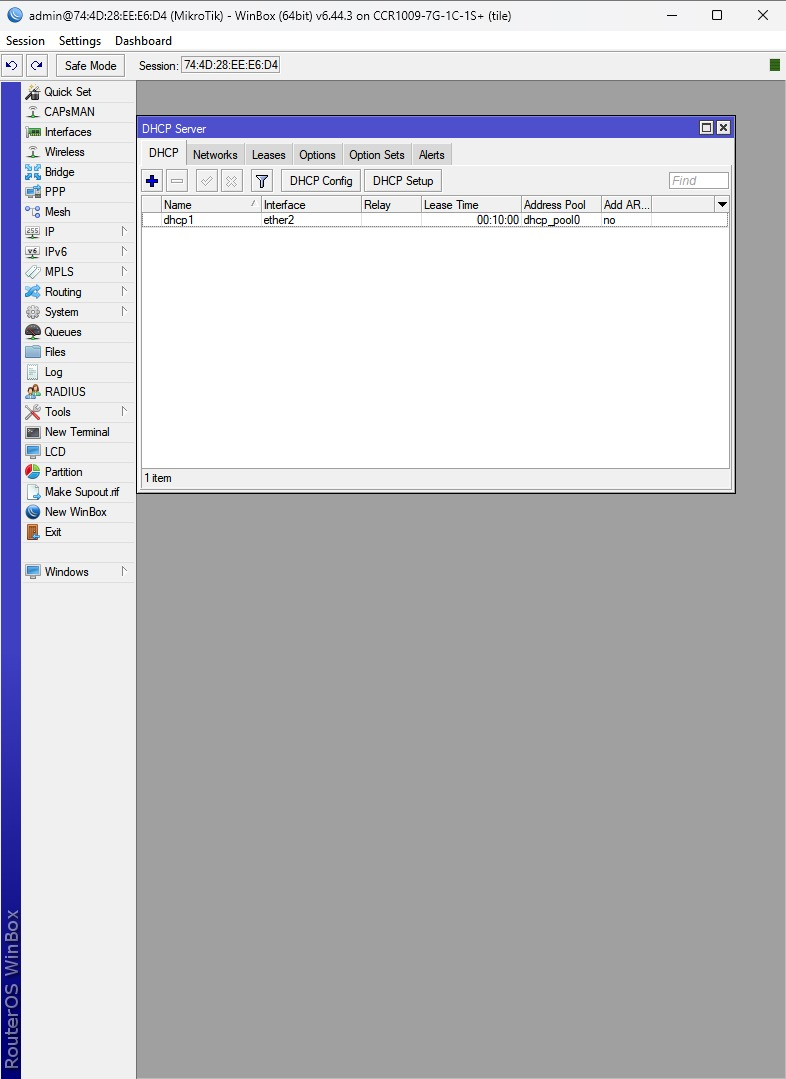
\includegraphics[width=0.7\textwidth]{img4/DHCPServer.jpeg}
        \caption{Jendela wizard "DHCP Setup" untuk antarmuka ether7}
    \end{figure}
    
    \item \textbf{Konfigurasi NAT:} Aturan NAT dibuat agar semua perangkat di jaringan lokal dapat mengakses internet menggunakan satu IP publik dari router.
    \begin{enumerate}
        \item Akses menu \textit{IP -> Firewall -> NAT}, lalu klik ikon `+`.
        \item Pada tab \textit{General}, atur \textit{Chain}: \textbf{src-nat}.
        \item Pada tab \textit{Action}, atur \textit{Action}: \textbf{masquerade}.
    \end{enumerate}
    \begin{figure}[H]
        \centering
        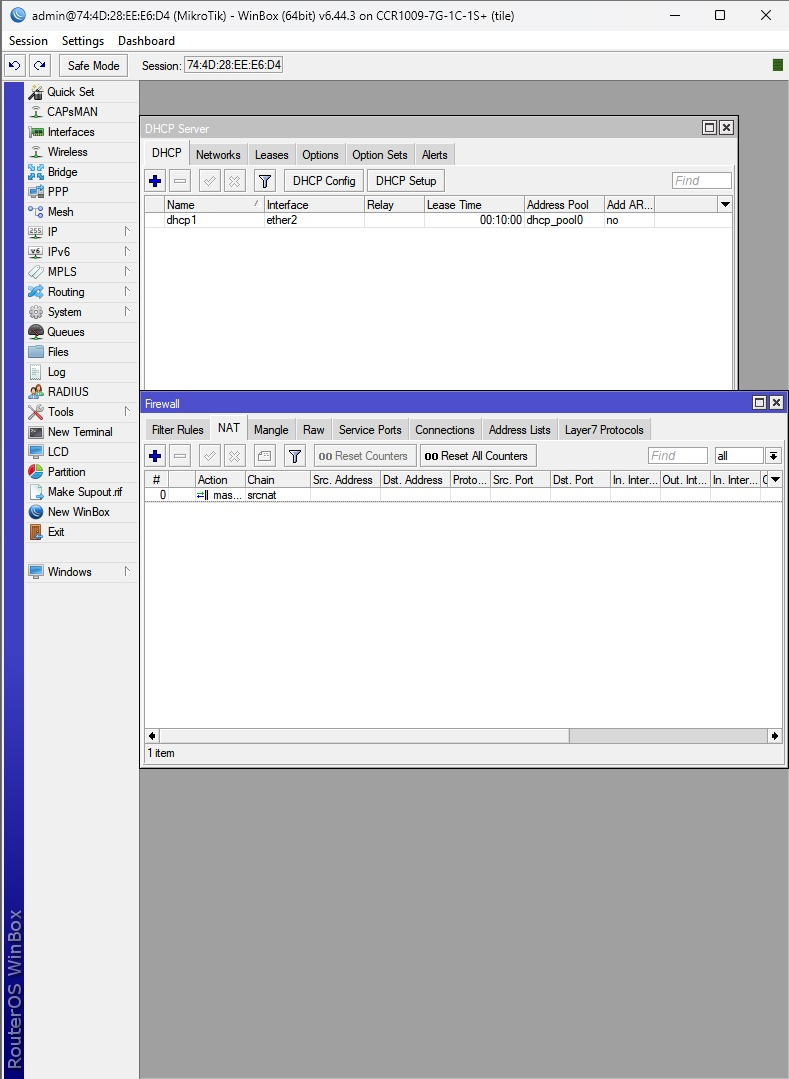
\includegraphics[width=0.7\textwidth]{img4/NATMasqueerade.jpeg}
        \caption{Konfigurasi aturan NAT Masquerade pada tab Action}
    \end{figure}
    
    \item \textbf{Uji Konektivitas NAT:} Dilakukan uji \texttt{ping} dari terminal Winbox ke server Google untuk memastikan router telah terhubung ke internet.
    \begin{figure}[H]
        \centering
        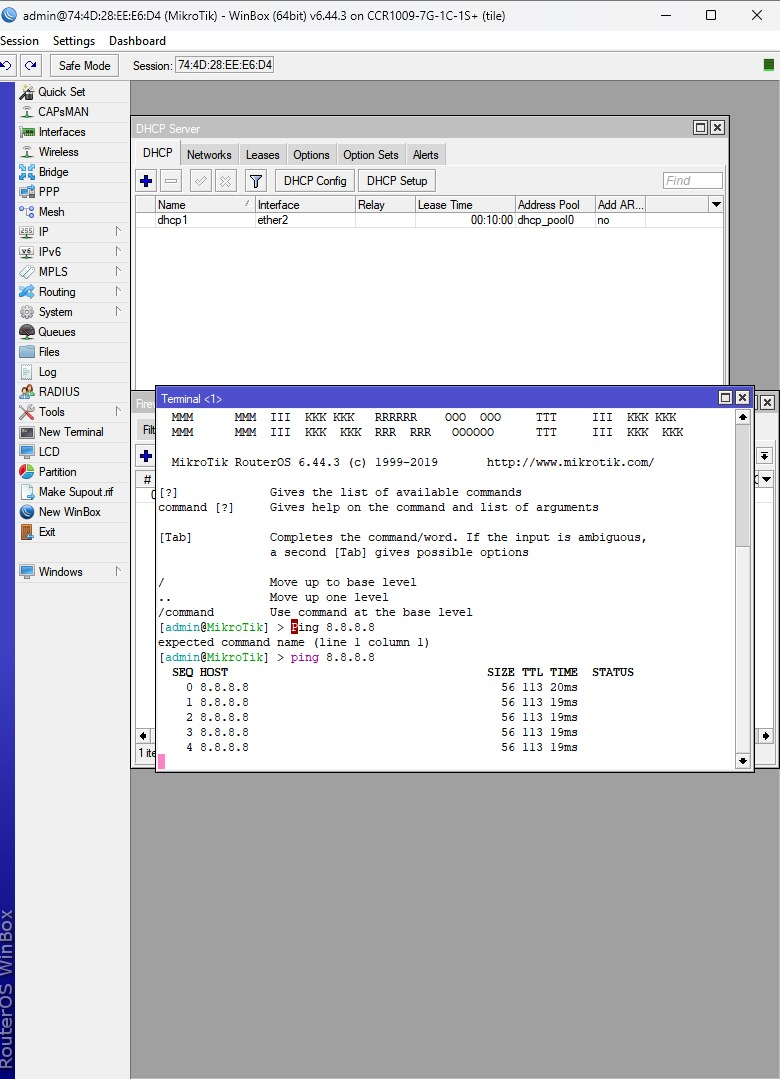
\includegraphics[width=0.6\textwidth]{img4/PingTestNat.jpeg}
        \caption{Hasil uji ping ke 8.8.8.8 yang berhasil setelah NAT dikonfigurasi}
    \end{figure}
\end{enumerate}

\subsection*{$\bullet$ Konfigurasi Aturan Firewall}
\addcontentsline{toc}{subsection}{Konfigurasi Aturan Firewall}
Dua aturan filter ditambahkan pada firewall untuk membatasi jenis lalu lintas data tertentu dari jaringan lokal.

\begin{enumerate}
    \item \textbf{Pemblokiran ICMP (Ping):} Aturan dibuat untuk memblokir semua lalu lintas ICMP yang berasal dari jaringan lokal.
    \begin{enumerate}
        \item Akses menu \textit{IP -> Firewall -> Filter Rules}, lalu klik `+`.
        \item \textit{Chain}: \textbf{forward}.
        \item \textit{Protocol}: \textbf{icmp}.
        \item \textit{In. Interface}: \texttt{ether7}.
        \item \textit{Action}: \textbf{drop}.
    \end{enumerate}
    \begin{figure}[H]
        \centering
        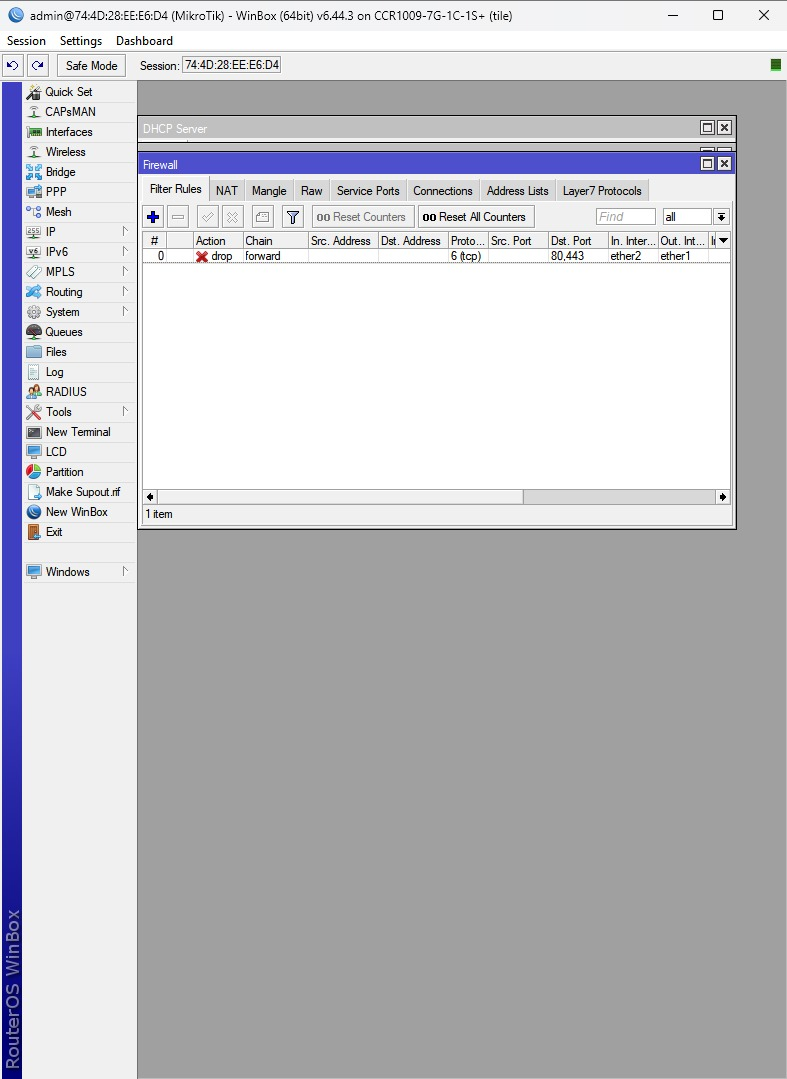
\includegraphics[width=0.7\textwidth]{img4/FireWallBlock.jpeg}
        \caption{Aturan firewall untuk melakukan "drop" pada protokol ICMP}
    \end{figure}
    
    \item \textbf{Pemblokiran Konten Website:} Aturan dibuat untuk memblokir akses ke situs web yang mengandung kata kunci "speedtest".
    \begin{enumerate}
        \item Buat aturan baru di \textit{Filter Rules}.
        \item \textit{Chain}: \textbf{forward}.
        \item \textit{Protocol}: \textbf{tcp}, dengan \textit{Dst. Port}: \texttt{80,443}.
        \item \textit{In. Interface}: \texttt{ether7} dan \textit{Out. Interface}: \texttt{ether1}.
        \item Pada tab \textit{Advanced}, atur \textit{Content}: \texttt{speedtest}.
        \item \textit{Action}: \textbf{drop}.
    \end{enumerate}
    \begin{figure}[H]
        \centering
        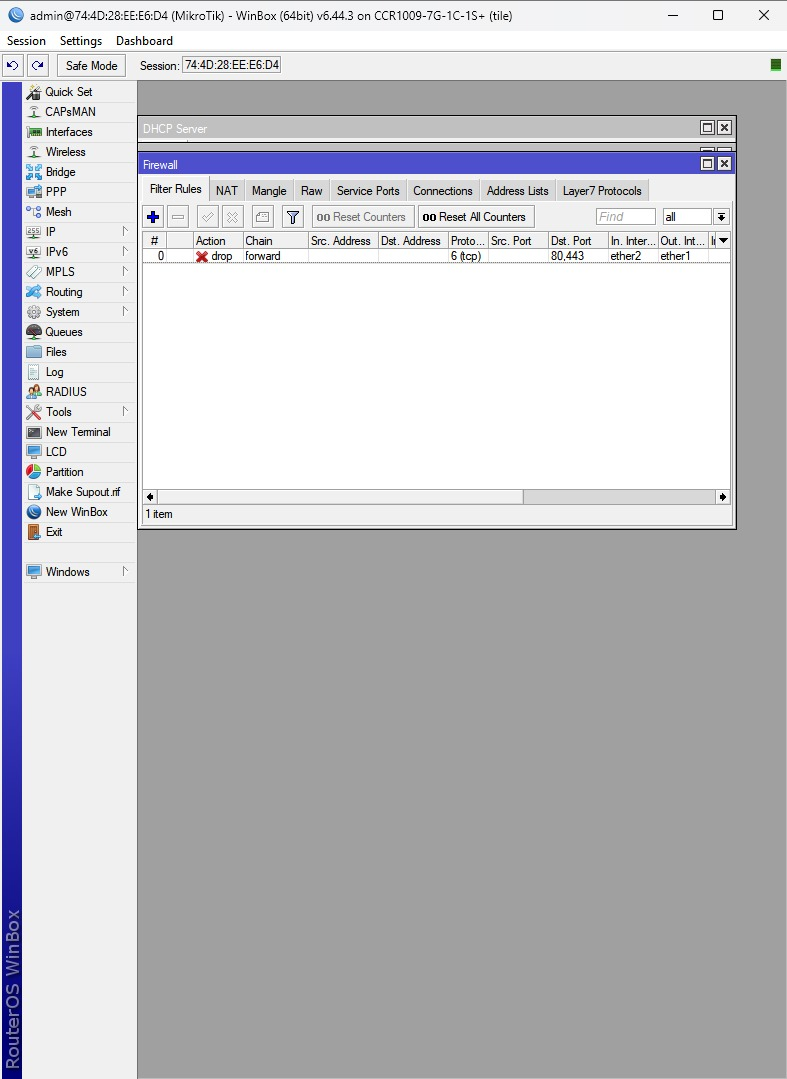
\includegraphics[width=0.7\textwidth]{img4/FireWallBlock.jpeg}
        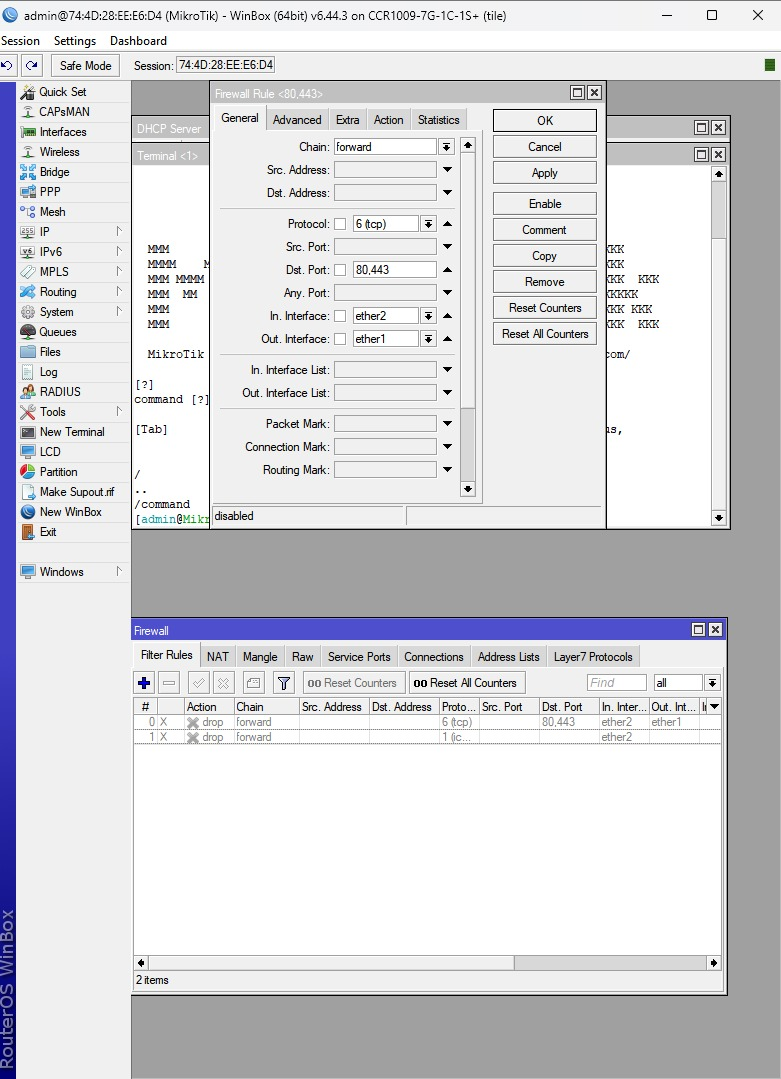
\includegraphics[width=0.7\textwidth]{img4/firewallblock.jpeg}
        \caption{Pengaturan pemblokiran konten pada tab Advanced}
    \end{figure}
\end{enumerate}

\subsection*{$\bullet$ Pengujian Fungsionalitas}
\addcontentsline{toc}{subsection}{Pengujian Fungsionalitas}
Pengujian akhir dilakukan dari sisi klien (laptop) untuk memverifikasi efektivitas aturan firewall yang telah dibuat.

\begin{enumerate}
    \item \textbf{Pengujian Blokir ICMP:} Perintah \texttt{ping 8.8.8.8} dijalankan dari Command Prompt laptop.
    \begin{figure}[H]
        \centering
        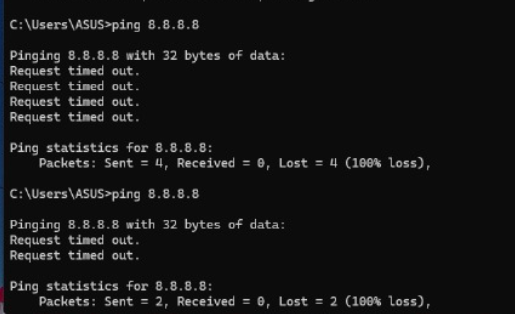
\includegraphics[width=0.6\textwidth]{img4/PingTestRTO.png}
        \caption{Hasil uji ping menunjukkan "Request Timed Out" saat aturan firewall ICMP aktif}
    \end{figure}
    \item Setelah aturan firewall ICMP dinonaktifkan (\textit{disable}), uji ping diulangi.
    \begin{figure}[H]
        \centering
        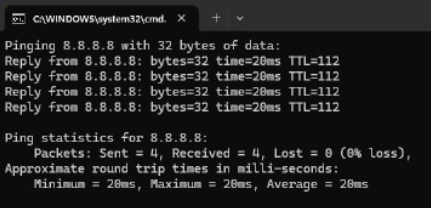
\includegraphics[width=0.6\textwidth]{img4/PingTestSuccess.png}
        \caption{Hasil uji ping berhasil setelah aturan firewall ICMP dinonaktifkan}
    \end{figure}
    
    \item \textbf{Pengujian Blokir Konten:} Dilakukan upaya untuk mengakses situs web \texttt{www.speedtest.net} dari peramban web.
    \begin{figure}[H]
        \centering
        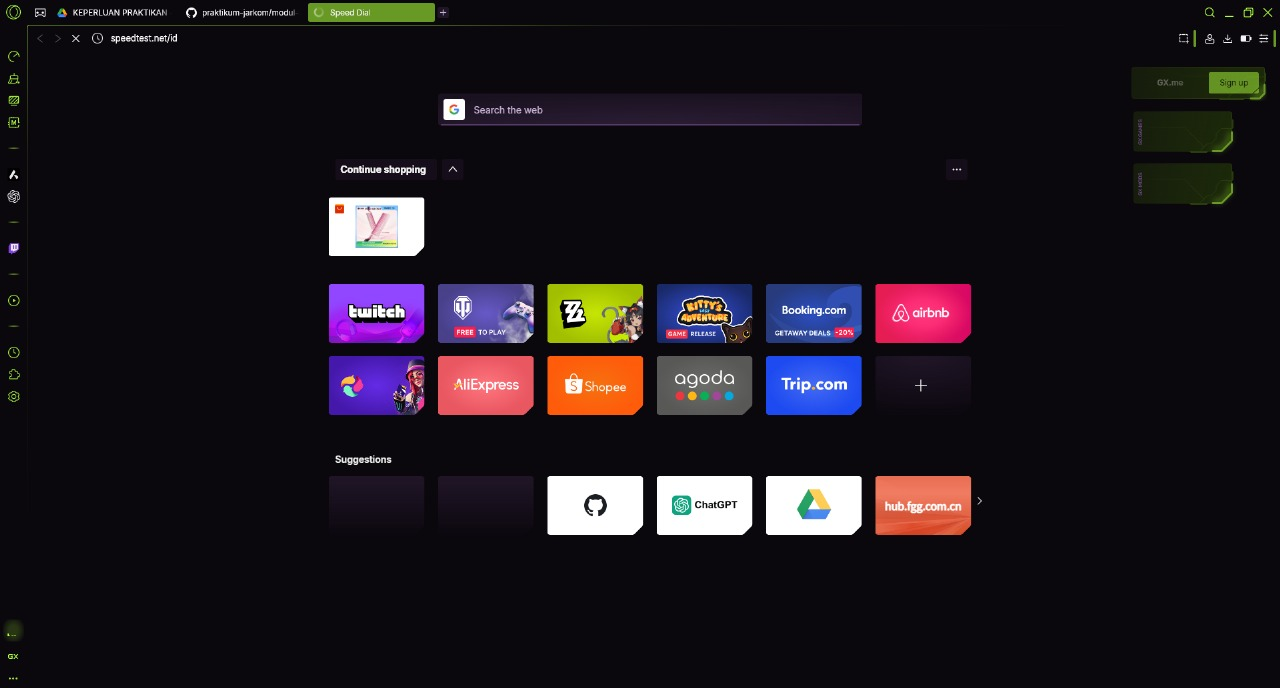
\includegraphics[width=0.7\textwidth]{img4/SpeedTestBlocker.jpeg}
        \caption{Peramban web gagal memuat situs saat aturan pemblokiran konten aktif}
    \end{figure}
    \item Setelah aturan pemblokiran konten dinonaktifkan, situs web yang sama dicoba diakses kembali.
\end{enumerate}

\newpage
\section{Analisis Hasil Percobaan}
\addcontentsline{toc}{section}{Analisis Hasil Percobaan}
Berdasarkan serangkaian langkah percobaan yang telah saya lakukan pada router MikroTik, saya melakukan analisis terhadap fungsionalitas dan hasil dari setiap konfigurasi yang diterapkan.

\subsection*{$\bullet$ Analisis Konfigurasi NAT}
\addcontentsline{toc}{subsection}{Analisis Konfigurasi NAT}
Pada percobaan ini, saya mengonfigurasi NAT menggunakan metode \textbf{masquerade}. Dari pengamatan saya, metode ini berhasil menyediakan konektivitas internet untuk seluruh perangkat di jaringan lokal (LAN). Keberhasilan ini disebabkan oleh cara kerja \textit{masquerade} yang secara dinamis dan otomatis menerjemahkan alamat IP privat dari jaringan lokal (misalnya \texttt{192.168.10.1}) menjadi satu alamat IP publik yang didapat oleh router pada antarmuka \texttt{ether1}. Ketika server di internet membalas, router menggunakan tabel pelacakan koneksi (\textit{connection tracking}) untuk mengetahui secara pasti ke perangkat privat mana paket balasan tersebut harus diteruskan. Hal ini terbukti dari uji \texttt{ping} ke \texttt{8.8.8.8} dari terminal router yang berhasil, menandakan router itu sendiri sudah terhubung ke internet dan siap meneruskan koneksi.

\subsection*{$\bullet$ Analisis Aturan Firewall ICMP}
\addcontentsline{toc}{subsection}{Analisis Aturan Firewall ICMP}
Saya membuat aturan firewall untuk memblokir protokol ICMP dengan aksi \textbf{drop}. Saat saya melakukan uji \texttt{ping} dari laptop klien, hasilnya adalah \textit{Request Timed Out} (RTO). Saya menganalisis bahwa kegagalan ping ini disebabkan oleh aksi \texttt{drop} yang saya pilih. Aksi ini secara diam-diam membuang paket ICMP yang masuk ke router dari jaringan lokal tanpa mengirimkan notifikasi error apapun kembali ke pengirim. Akibatnya, laptop saya sebagai pengirim hanya bisa menunggu balasan yang tidak akan pernah datang hingga batas waktu habis. Ini berbeda dengan aksi \texttt{reject}, yang akan secara aktif mengirimkan balasan "Destination Unreachable". Keberhasilan uji \texttt{ping} setelah aturan ini dinonaktifkan mengonfirmasi bahwa aturan tersebut bekerja sesuai fungsinya.

\subsection*{$\bullet$ Analisis Aturan Firewall Pemblokiran Konten}
\addcontentsline{toc}{subsection}{Analisis Aturan Firewall Pemblokiran Konten}
Aturan pemblokiran konten yang menargetkan kata kunci \texttt{speedtest} juga berhasil saya implementasikan. Aturan ini bekerja pada Layer 7 model OSI, di mana router secara aktif memeriksa aliran data dari paket TCP yang menuju port 80 (HTTP) dan 443 (HTTPS). Ketika string \texttt{speedtest} terdeteksi dalam data (misalnya, dalam nama domain atau konten halaman), firewall akan langsung memutuskan koneksi dengan aksi \texttt{drop}. Inilah sebabnya saat saya mencoba mengakses situs \texttt{www.speedtest.net}, peramban web hanya terus memuat tanpa menampilkan konten apapun. Situs tersebut baru dapat diakses dengan normal setelah aturan filter ini saya nonaktifkan, yang membuktikan efektivitas pemfilteran berbasis konten.

\newpage
\section{Tugas Modul}
\addcontentsline{toc}{section}{Tugas Modul}
Pada bagian ini, saya melakukan simulasi jaringan menggunakan Cisco Packet Tracer untuk menerapkan konsep NAT dan berbagai skenario firewall menggunakan Access Control List (ACL) pada topologi yang telah ditentukan.

\subsection*{$\bullet$ Topologi dan Konfigurasi Awal}
\addcontentsline{toc}{subsection}{Topologi dan Konfigurasi Awal}
Langkah awal adalah membangun topologi jaringan dan melakukan konfigurasi IP dasar pada setiap perangkat.
\begin{enumerate}
    \item \textbf{Pembuatan Topologi Jaringan:} Saya menempatkan 1 Router, 1 Switch, 3 PC, dan 1 Server pada workspace Cisco Packet Tracer dan menghubungkannya dengan kabel yang sesuai. Pengkabelan ini mengikuti praktik terbaik, di mana port FastEthernet pada switch digunakan untuk PC, dan port GigabitEthernet digunakan untuk koneksi uplink ke router.
    \begin{figure}[H]
        \centering
        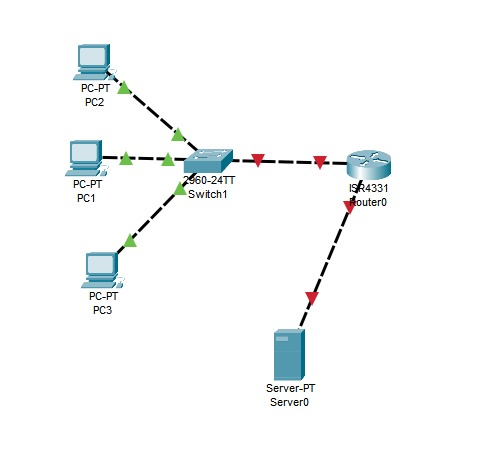
\includegraphics[width=0.7\textwidth]{img4/topoawal.jpeg}
        \caption{Topologi awal jaringan sebelum konfigurasi.}
    \end{figure}
    
    \item \textbf{Konfigurasi Alamat IP Perangkat:} Setiap perangkat dikonfigurasi dengan alamat IP statis sesuai skema pengalamatan yang telah dirancang. Hal ini penting agar setiap perangkat memiliki identitas yang jelas di dalam jaringannya masing-masing dan untuk mempermudah proses pembuatan aturan firewall nanti.
    
    \begin{figure}[H]
        \centering
        \begin{minipage}{0.32\textwidth}
            \centering
            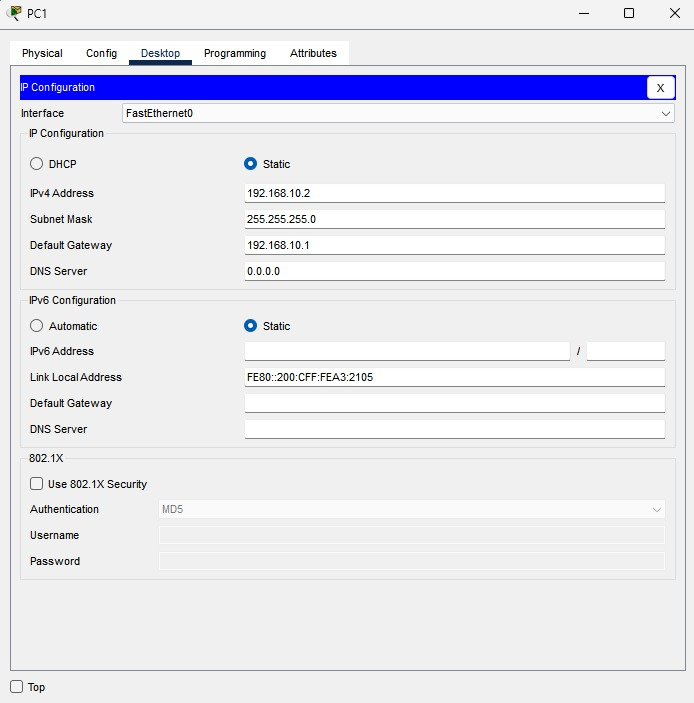
\includegraphics[width=\textwidth]{img4/IPCPC1.jpeg}
            \caption*{(a) IP PC1}
        \end{minipage}\hfill
        \begin{minipage}{0.32\textwidth}
            \centering
            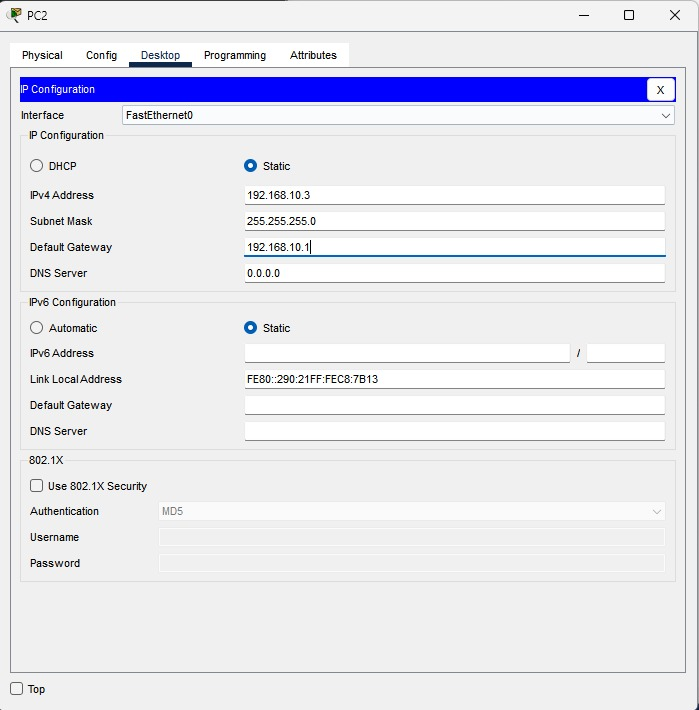
\includegraphics[width=\textwidth]{img4/IPCPC2.jpeg}
            \caption*{(b) IP PC2}
        \end{minipage}\hfill
        \begin{minipage}{0.32\textwidth}
            \centering
            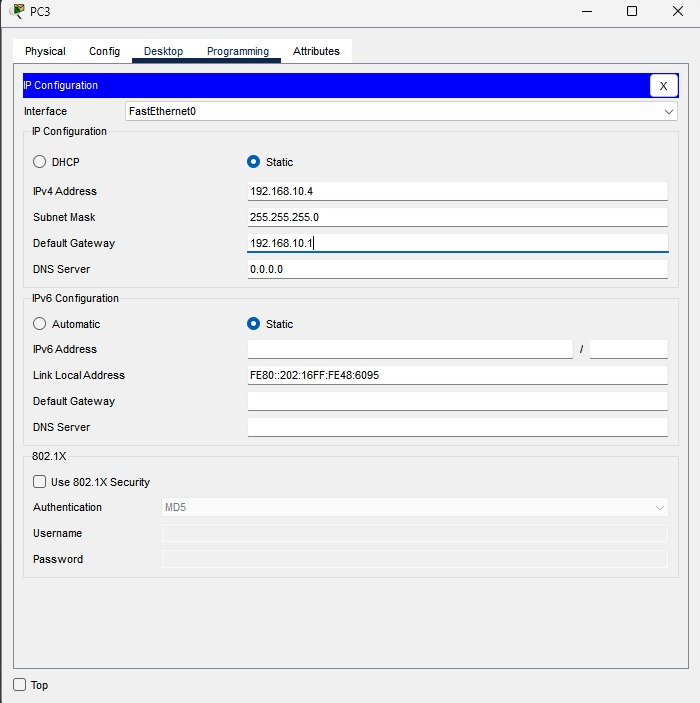
\includegraphics[width=\textwidth]{img4/IPCPC3.jpeg}
            \caption*{(c) IP PC3}
        \end{minipage}
        \vspace{1em}
        \begin{minipage}{0.48\textwidth}
            \centering
            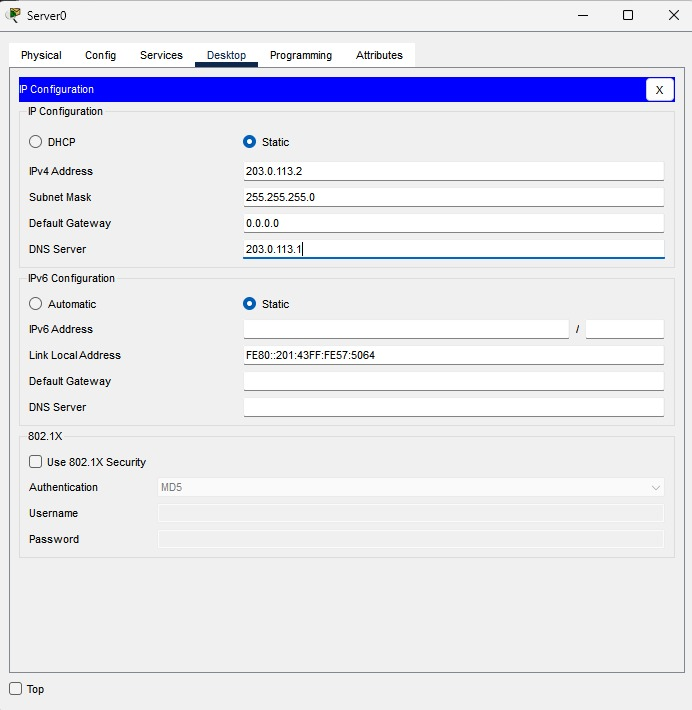
\includegraphics[width=0.7\textwidth]{img4/IPCServer.jpeg}
            \caption*{(d) IP Server}
        \end{minipage}\hfill
        \begin{minipage}{0.48\textwidth}
            \centering
            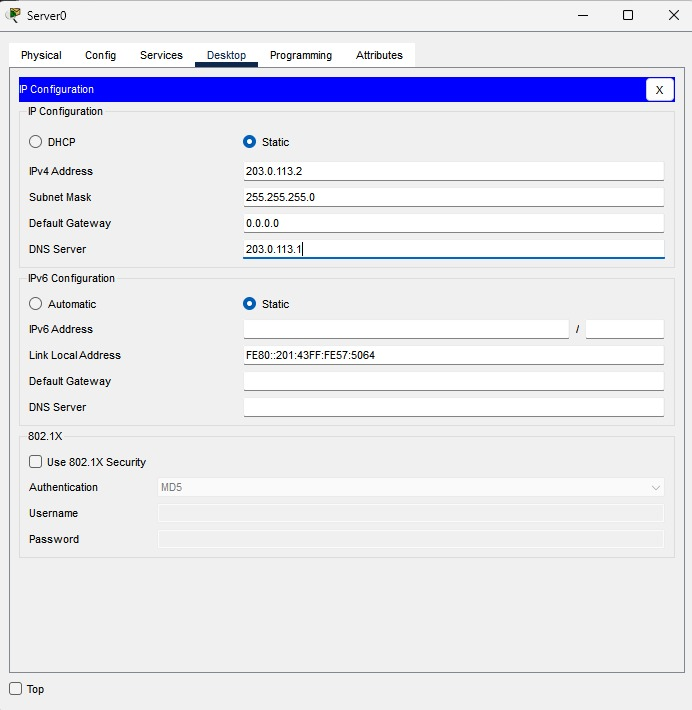
\includegraphics[width=0.7\textwidth]{img4/IPCServer.jpeg}
            \caption*{(e) IP Router via CLI}
        \end{minipage}
        \caption{Kolase konfigurasi IP pada (a) PC1, (b) PC2, (c) PC3, (d) Server, dan (e) antarmuka Router.}
    \end{figure}
    
    \begin{figure}[H]
        \centering
        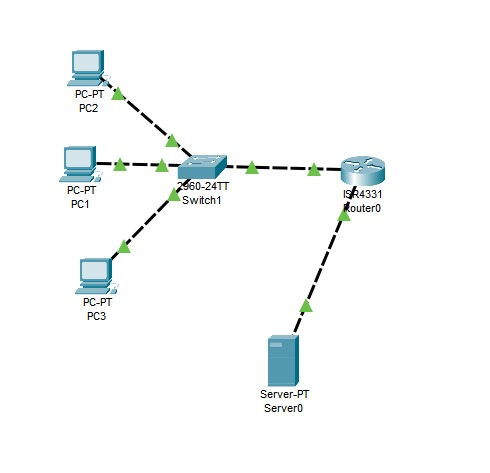
\includegraphics[width=0.65\textwidth]{img4/topoconnect.jpeg}
        \caption{Topologi jaringan setelah semua perangkat terhubung.}
    \end{figure}

    \item \textbf{Verifikasi Konektivitas Awal:} Setelah semua IP diatur, saya melakukan uji \texttt{ping} untuk memverifikasi konektivitas. Sesuai asumsi, ping antar PC dalam satu LAN berhasil karena mereka terhubung melalui switch pada segmen jaringan yang sama. Namun, ping dari PC ke Server gagal. Ini terjadi karena belum ada NAT; server di jaringan publik tidak tahu cara mengirim balasan ke alamat IP privat \texttt{192.168.10.2}.
    \begin{figure}[H]
        \centering
        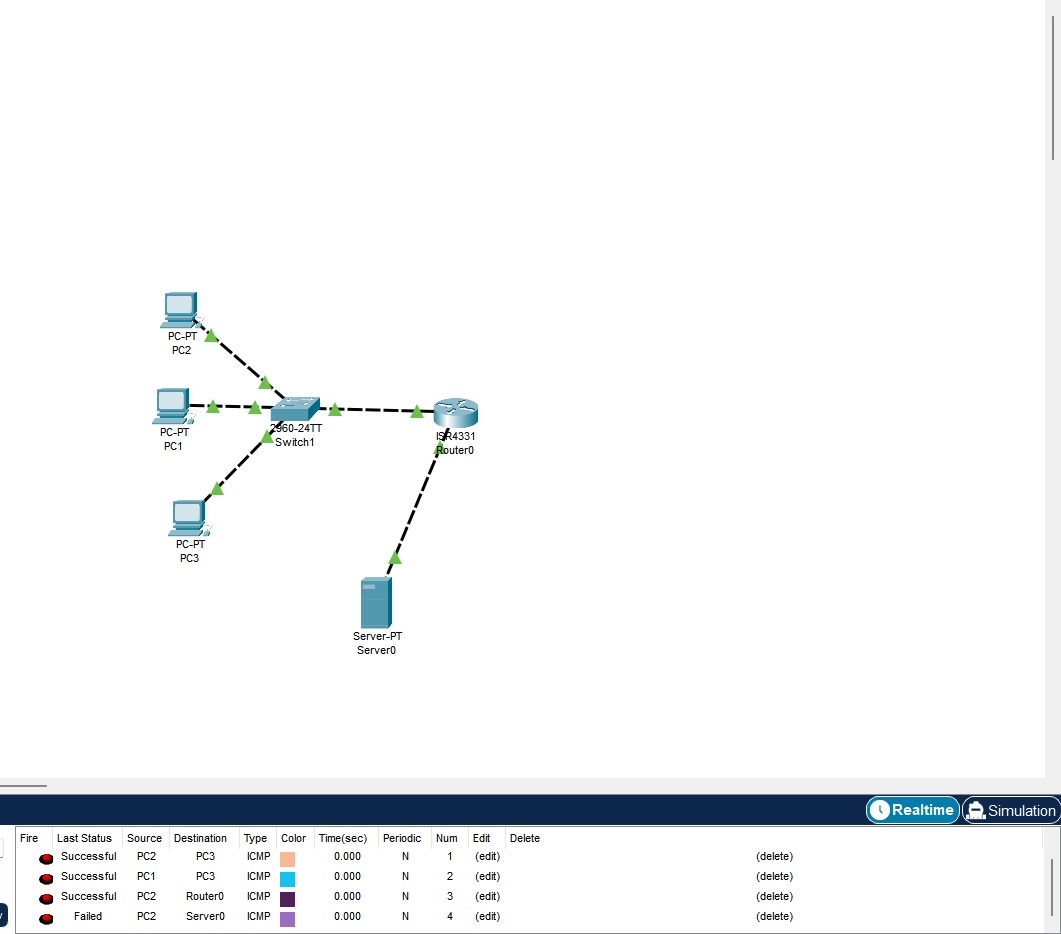
\includegraphics[width=0.7\textwidth]{img4/CiscPingServerNo.jpeg}
        \caption{Hasil ping: sukses antar PC di LAN, gagal dari PC ke Server.}
    \end{figure}
\end{enumerate}

\subsection*{$\bullet$ Implementasi NAT Overload}
\addcontentsline{toc}{subsection}{Implementasi NAT Overload}
Untuk mengatasi masalah konektivitas ke server, saya mengimplementasikan NAT Overload (PAT).
\begin{enumerate}
    \setcounter{enumi}{3}
    \item \textbf{Definisi Antarmuka NAT:} Langkah pertama adalah memberitahu router mana antarmuka yang menghadap ke dalam (LAN) dan mana yang ke luar (Publik). Saya menetapkan \texttt{GigabitEthernet0/0/0} sebagai \texttt{ip nat inside} dan \texttt{GigabitEthernet0/0/1} sebagai \texttt{ip nat outside}.
    \begin{figure}[H]
        \centering
        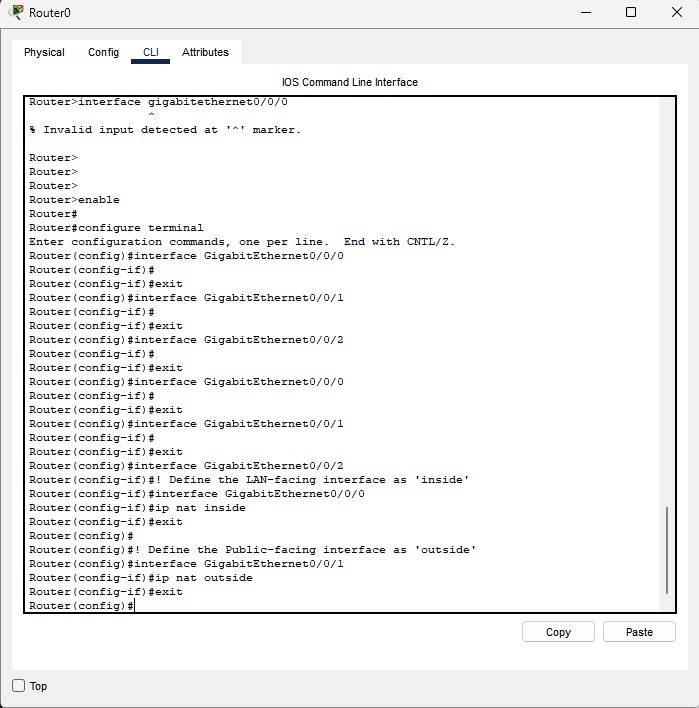
\includegraphics[width=0.7\textwidth]{img4/NATInterface.jpeg}
        \caption{Konfigurasi antarmuka NAT inside dan outside.}
    \end{figure}
    
    \item \textbf{Pembuatan Aturan NAT:} Saya membuat ACL (\texttt{access-list 1}) untuk mengidentifikasi trafik dari LAN yang boleh ditranslasikan, kemudian mengikatnya ke antarmuka publik dengan perintah \texttt{ip nat inside source list 1 interface ... overload}. Ini adalah inti dari konfigurasi NAT.
    \begin{figure}[H]
        \centering
        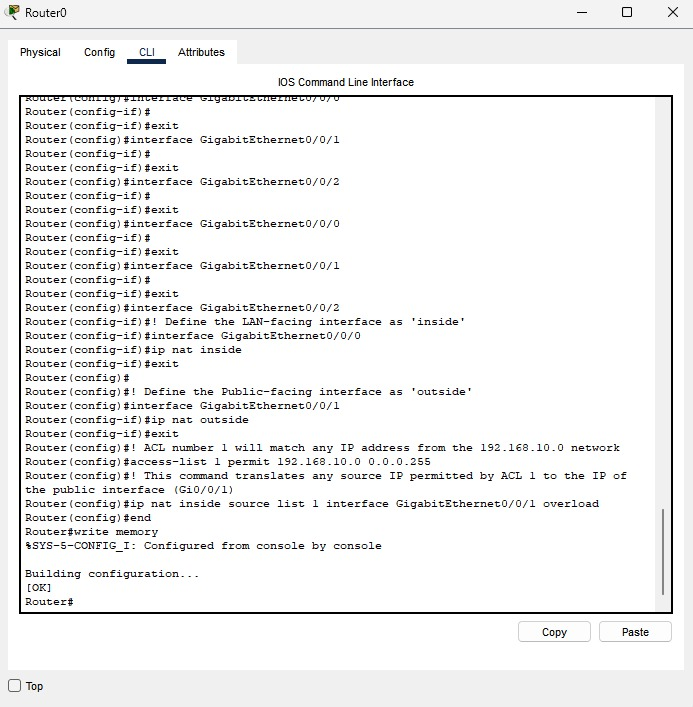
\includegraphics[width=0.7\textwidth]{img4/NATrule.jpeg}
        \caption{Perintah untuk membuat ACL dan aturan NAT Overload.}
    \end{figure}
    
    \item \textbf{Pengujian Setelah NAT:} Setelah NAT aktif, saya kembali melakukan uji \texttt{ping} dari setiap PC ke Server. Hasilnya, semua ping berhasil. Ini membuktikan bahwa NAT telah bekerja dengan benar, menerjemahkan alamat IP privat setiap PC menjadi alamat IP publik router.
    \begin{figure}[H]
        \centering
        \begin{minipage}{0.48\textwidth}
            \centering
            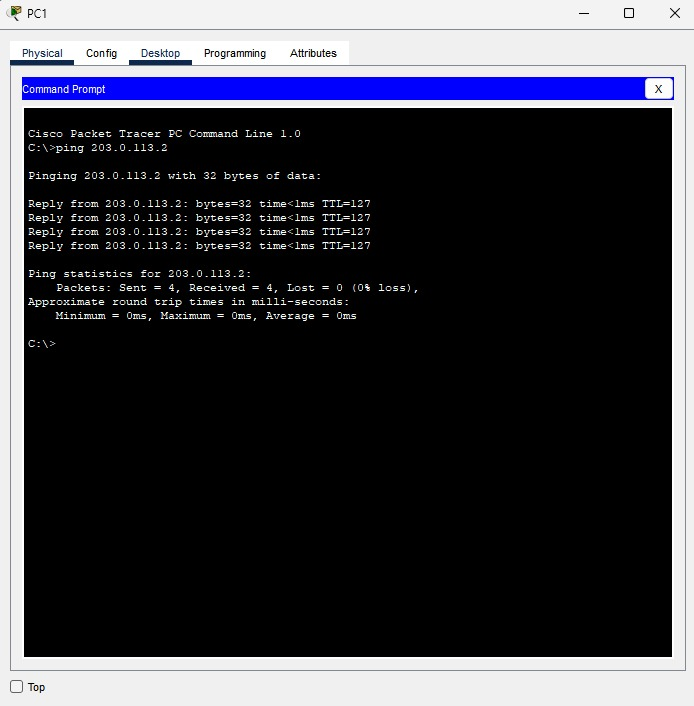
\includegraphics[width=0.8\textwidth]{img4/NATpingpc1.jpeg}
            \caption*{(a) Ping PC1 ke Server}
        \end{minipage}\hfill
        \begin{minipage}{0.48\textwidth}
            \centering
            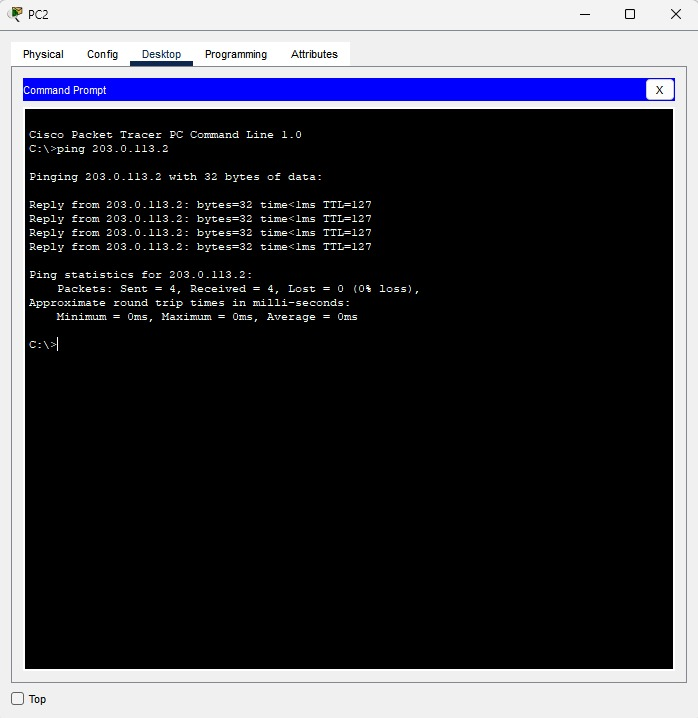
\includegraphics[width=0.8\textwidth]{img4/NATpingpc2.jpeg}
            \caption*{(b) Ping PC2 ke Server}
        \end{minipage}
        \vspace{1em}
        \begin{minipage}{0.48\textwidth}
            \centering
            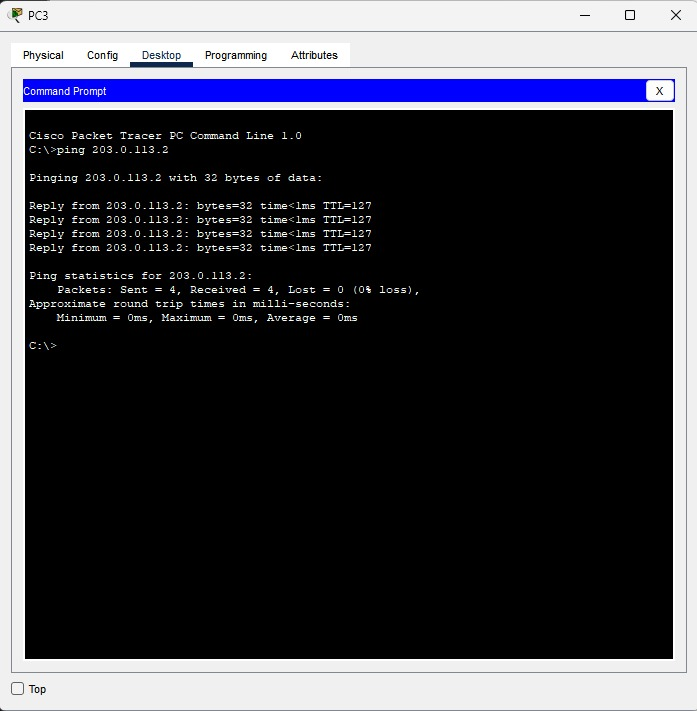
\includegraphics[width=0.8\textwidth]{img4/NATpingpc3.jpeg}
            \caption*{(c) Ping PC3 ke Server}
        \end{minipage}
        \caption{Uji konektivitas setelah NAT aktif menunjukkan semua PC dapat terhubung ke Server.}
    \end{figure}
\end{enumerate}

\subsection*{$\bullet$ Skenario Firewall 1: Izinkan Hanya PC1}
\addcontentsline{toc}{subsection}{Skenario Firewall 1: Izinkan Hanya PC1}
Skenario pertama adalah menerapkan kebijakan keamanan di mana hanya PC1 yang diizinkan mengakses Server.
\begin{enumerate}
    \setcounter{enumi}{6}
    \item \textbf{Pembuatan ACL Skenario 1:} Saya membuat \texttt{access-list 20} yang hanya berisi satu baris perintah: \texttt{permit host 192.168.10.2}. ACL ini memiliki sifat "implicit deny" di akhir, yang berarti semua trafik lain yang tidak cocok dengan aturan permit ini akan otomatis ditolak. Aturan ini kemudian saya terapkan secara \textit{inbound} pada antarmuka LAN router.
    \begin{figure}[H]
        \centering
        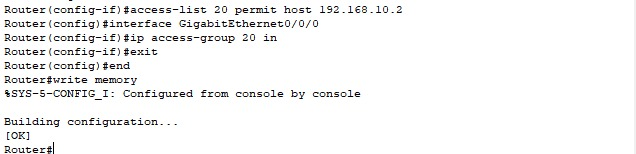
\includegraphics[width=0.7\textwidth]{img4/CiscACL20.jpeg}
        \caption{Konfigurasi ACL 20 untuk mengizinkan hanya PC1.}
    \end{figure}
    
    \item \textbf{Pengujian Skenario 1:} Hasil pengujian sesuai dengan yang diharapkan. Ping dari PC1 berhasil, sementara ping dari PC2 dan PC3 gagal. Uji ping antar PC di LAN juga tetap berhasil, membuktikan bahwa ACL yang diterapkan pada router tidak mengganggu komunikasi lokal yang tidak melewati router.
    \begin{figure}[H]
        \centering
        \begin{minipage}{0.48\textwidth}
            \centering
            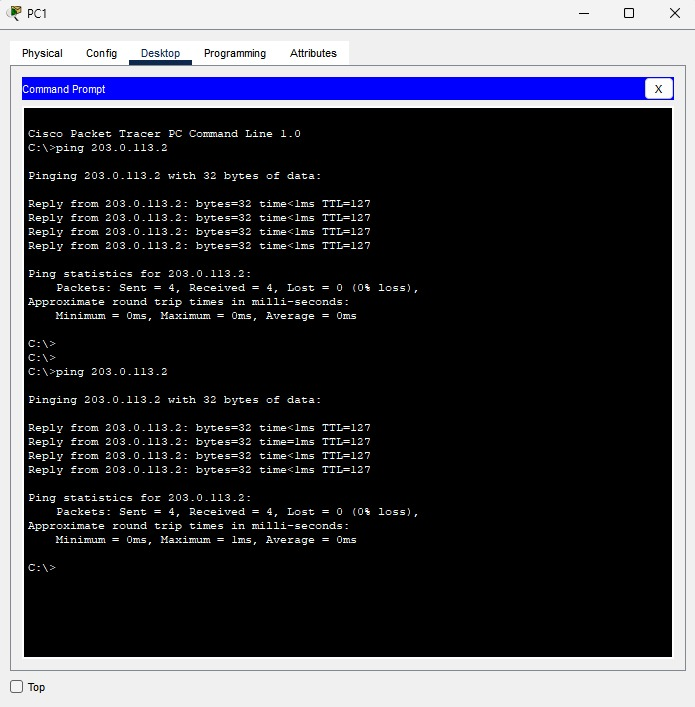
\includegraphics[width=0.8\textwidth]{img4/PC1Ping.jpeg}
            \caption*{(a) PC1 ke Server (Success)}
        \end{minipage}\hfill
        \begin{minipage}{0.48\textwidth}
            \centering
            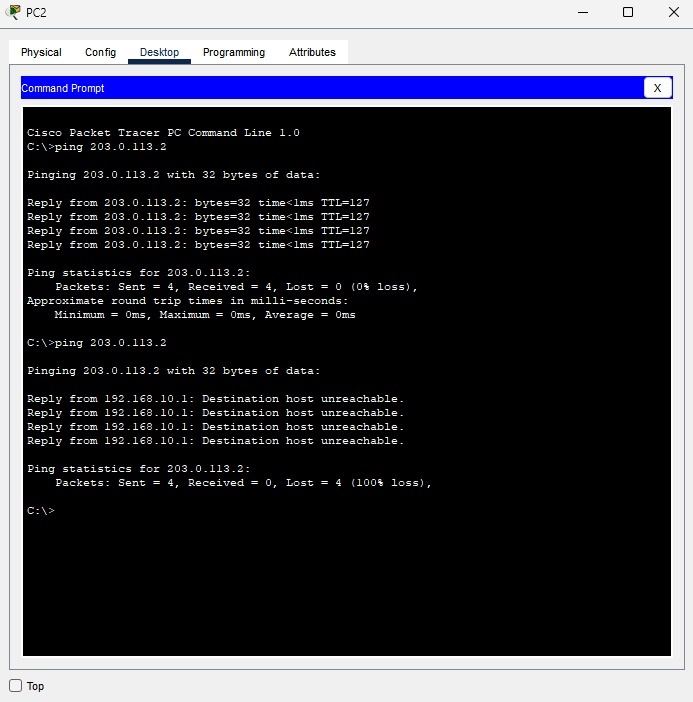
\includegraphics[width=0.8\textwidth]{img4/PC2Ping.jpeg}
            \caption*{(b) PC2 ke Server (Failed)}
        \end{minipage}
        \vspace{1em}
        \begin{minipage}{0.48\textwidth}
            \centering
            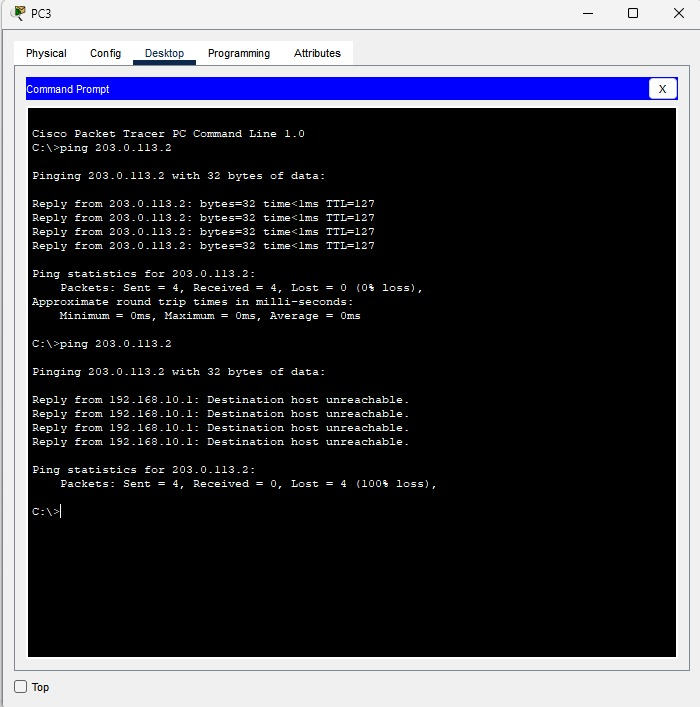
\includegraphics[width=0.8\textwidth]{img4/PC3Ping.jpeg}
            \caption*{(c) PC3 ke Server (Failed)}
        \end{minipage}\hfill
        \begin{minipage}{0.48\textwidth}
            \centering
            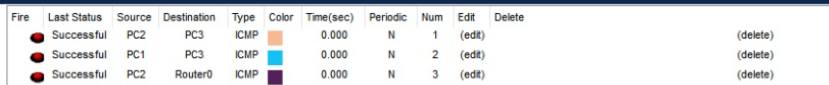
\includegraphics[width=0.8\textwidth]{img4/PingLan.png}
            \caption*{(d) PC2 ke PC3 (Success)}
        \end{minipage}
        \caption{Hasil pengujian ACL Skenario 1.}
    \end{figure}
\end{enumerate}

\subsection*{$\bullet$ Skenario Firewall 2: Blokir PC2 dan PC3}
\addcontentsline{toc}{subsection}{Skenario Firewall 2: Blokir PC2 dan PC3}
Skenario kedua adalah menerapkan kebijakan yang secara eksplisit memblokir PC2 dan PC3.
\begin{enumerate}
    \setcounter{enumi}{8}
    \item \textbf{Perubahan Konfigurasi ACL:} Pertama, saya membersihkan konfigurasi ACL sebelumnya. Kemudian saya membuat \texttt{access-list 30} dengan urutan: dua baris \texttt{deny} untuk PC2 dan PC3, diikuti satu baris \texttt{permit any} untuk mengizinkan semua trafik lainnya (termasuk PC1). Proses ini diverifikasi menggunakan perintah \texttt{show}.
     \begin{figure}[H]
        \centering
        \begin{minipage}{0.32\textwidth}
            \centering
            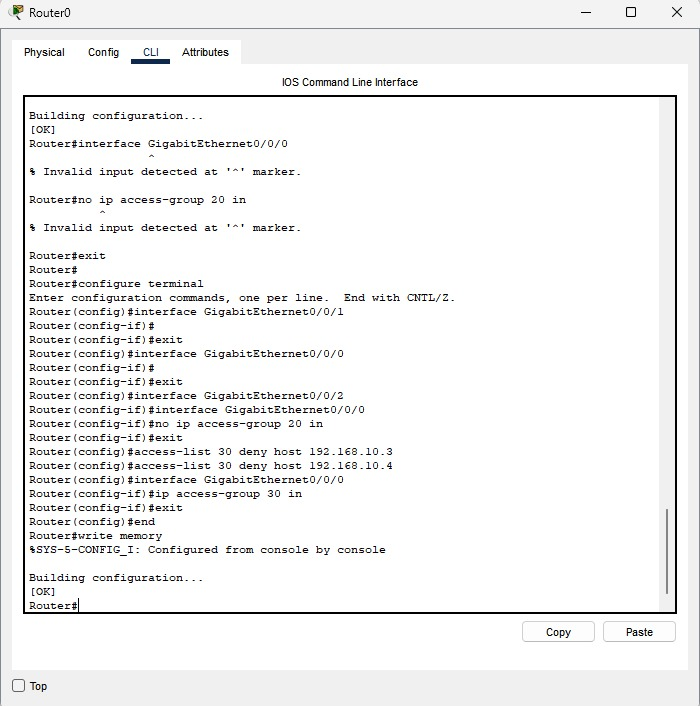
\includegraphics[width=\textwidth]{img4/removeACL30.jpeg}
            \caption*{(a) Hapus ACL lama}
        \end{minipage}\hfill
        \begin{minipage}{0.32\textwidth}
            \centering
            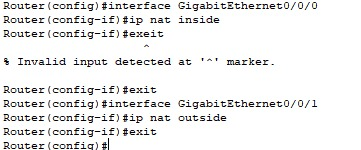
\includegraphics[width=\textwidth]{img4/AddACL30.jpeg}
            \caption*{(b) Buat ACL baru}
        \end{minipage}\hfill
        \begin{minipage}{0.32\textwidth}
            \centering
            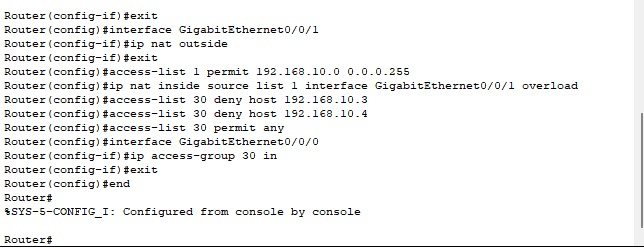
\includegraphics[width=\textwidth]{img4/ApplyACL30.jpeg}
            \caption*{(c) Terapkan ACL}
        \end{minipage}
        \vspace{1em} 
        \begin{minipage}{0.48\textwidth}
            \centering
            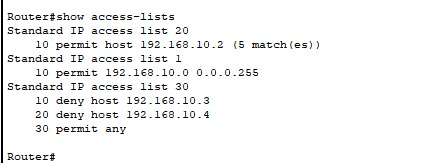
\includegraphics[width=0.8\textwidth]{img4/Verifconf.jpeg}
            \caption*{(d) Verifikasi `show access-lists`}
        \end{minipage}\hfill
        \begin{minipage}{0.48\textwidth}
            \centering
            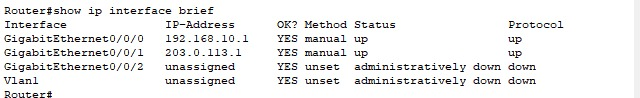
\includegraphics[width=0.8\textwidth]{img4/VerifInt.jpeg}
            \caption*{(e) Verifikasi `show ip int brief`}
        \end{minipage}
        \caption{Langkah-langkah perubahan konfigurasi ACL untuk Skenario 2.}
    \end{figure}
    
    \item \textbf{Pengujian Skenario 2:} Pengujian akhir dilakukan dan hasilnya kembali sesuai dengan konfigurasi. PC1 berhasil terhubung karena trafiknya lolos dari aturan \texttt{deny} dan diizinkan oleh \texttt{permit any}. Sementara itu, PC2 dan PC3 gagal karena trafik mereka cocok dengan aturan \texttt{deny} pertama yang ditemui oleh router.
    \begin{figure}[H]
        \centering
        \begin{minipage}{0.48\textwidth}
            \centering
            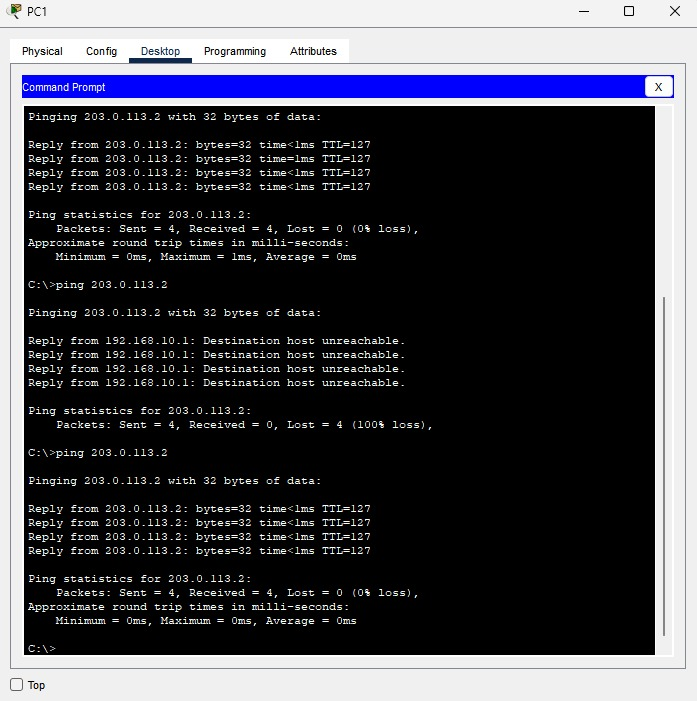
\includegraphics[width=0.8\textwidth]{img4/PC1ping2.jpeg}
            \caption*{(a) PC1 ke Server (Success)}
        \end{minipage}\hfill
        \begin{minipage}{0.48\textwidth}
            \centering
            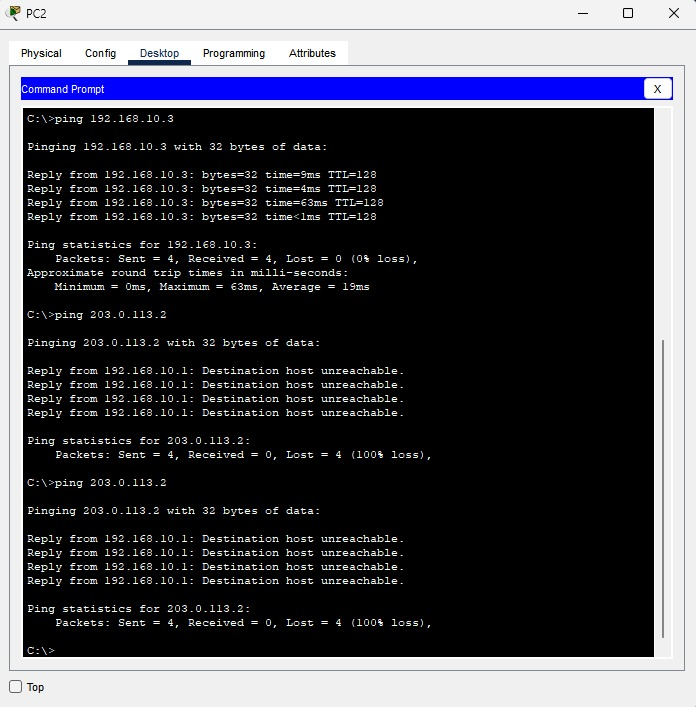
\includegraphics[width=0.8\textwidth]{img4/PC2ping2.jpeg}
            \caption*{(b) PC2 ke Server (Failed)}
        \end{minipage}
        \vspace{1em}
        \begin{minipage}{0.48\textwidth}
            \centering
            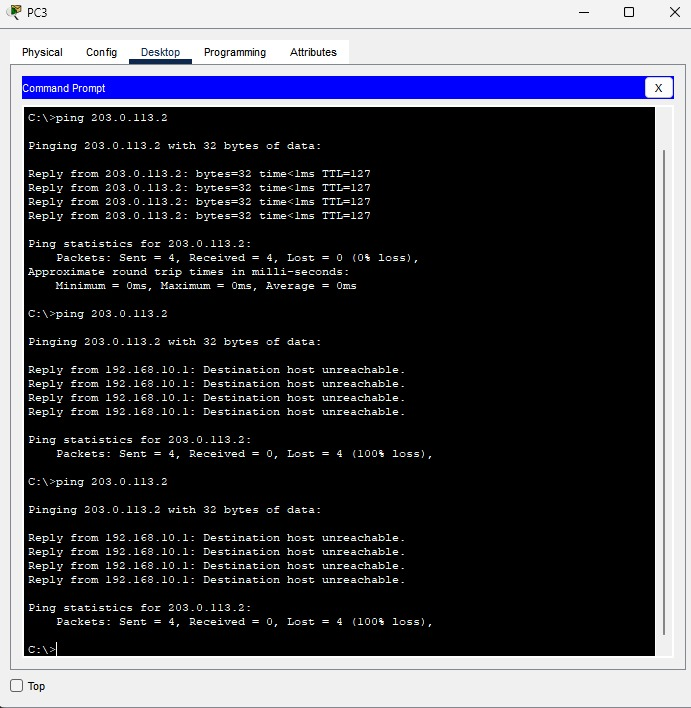
\includegraphics[width=0.8\textwidth]{img4/PC3ping2.jpeg}
            \caption*{(c) PC3 ke Server (Failed)}
        \end{minipage}
        \caption{Hasil pengujian akhir setelah ACL diubah untuk memblokir PC2 dan PC3.}
    \end{figure}
\end{enumerate}

\newpage
\section{Kesimpulan}
\addcontentsline{toc}{section}{Kesimpulan}

Melalui serangkaian percobaan dan simulasi pada praktikum ini, saya telah berhasil mengimplementasikan dan menganalisis dua konsep inti jaringan komputer, yaitu Network Address Translation (NAT) dan Firewall. Saya memahami bahwa NAT, khususnya melalui metode PAT (`masquerade` pada MikroTik dan `overload` pada Cisco), merupakan solusi fundamental untuk mengatasi kelangkaan alamat IPv4 dan berfungsi sebagai gerbang utama bagi jaringan lokal untuk dapat mengakses internet secara bersamaan. Implementasi yang berhasil pada kedua platform menunjukkan peran universal dan krusial dari teknologi ini dalam arsitektur jaringan modern.

Selanjutnya, pada topik Firewall, saya mendapatkan pemahaman mendalam mengenai pentingnya keamanan berlapis. Melalui praktikum MikroTik, saya belajar cara memfilter lalu lintas tidak hanya berdasarkan protokol Layer 4 seperti ICMP, tetapi juga hingga ke Layer 7 dengan memblokir akses berdasarkan konten spesifik dari sebuah situs web. Sementara itu, pada Tugas Modul simulasi Cisco, saya mendalami penggunaan Access Control List (ACL) sebagai fondasi firewall. Dari simulasi tersebut, saya dapat menyimpulkan bahwa efektivitas sebuah ACL sangat bergantung pada logika dan urutan aturan (`rule order`), pemahaman akan `implicit deny` yang secara default menolak semua lalu lintas yang tidak diizinkan secara eksplisit, serta penempatan aturan (`inbound` atau `outbound`) yang strategis untuk mengontrol alur data secara efisien tanpa mengganggu komunikasi internal di dalam LAN.

Secara keseluruhan, praktikum ini memberikan pengetahuan praktis yang komprehensif, membuktikan bahwa jika NAT adalah kunci untuk konektivitas, maka Firewall yang terkonfigurasi dengan baik adalah pilar keamanannya, di mana keduanya harus bekerja secara sinergis untuk menciptakan lingkungan jaringan yang fungsional sekaligus aman.
\newpage
\section{Lampiran}
\subsection*{Dokumentasi saat praktikum}
\addcontentsline{toc}{subsection}{Dokumentasi saat praktikum}
Berikut adalah dokumentasi saat praktikum Modul 4 berlangsung.

\begin{figure}[H]
    \centering
    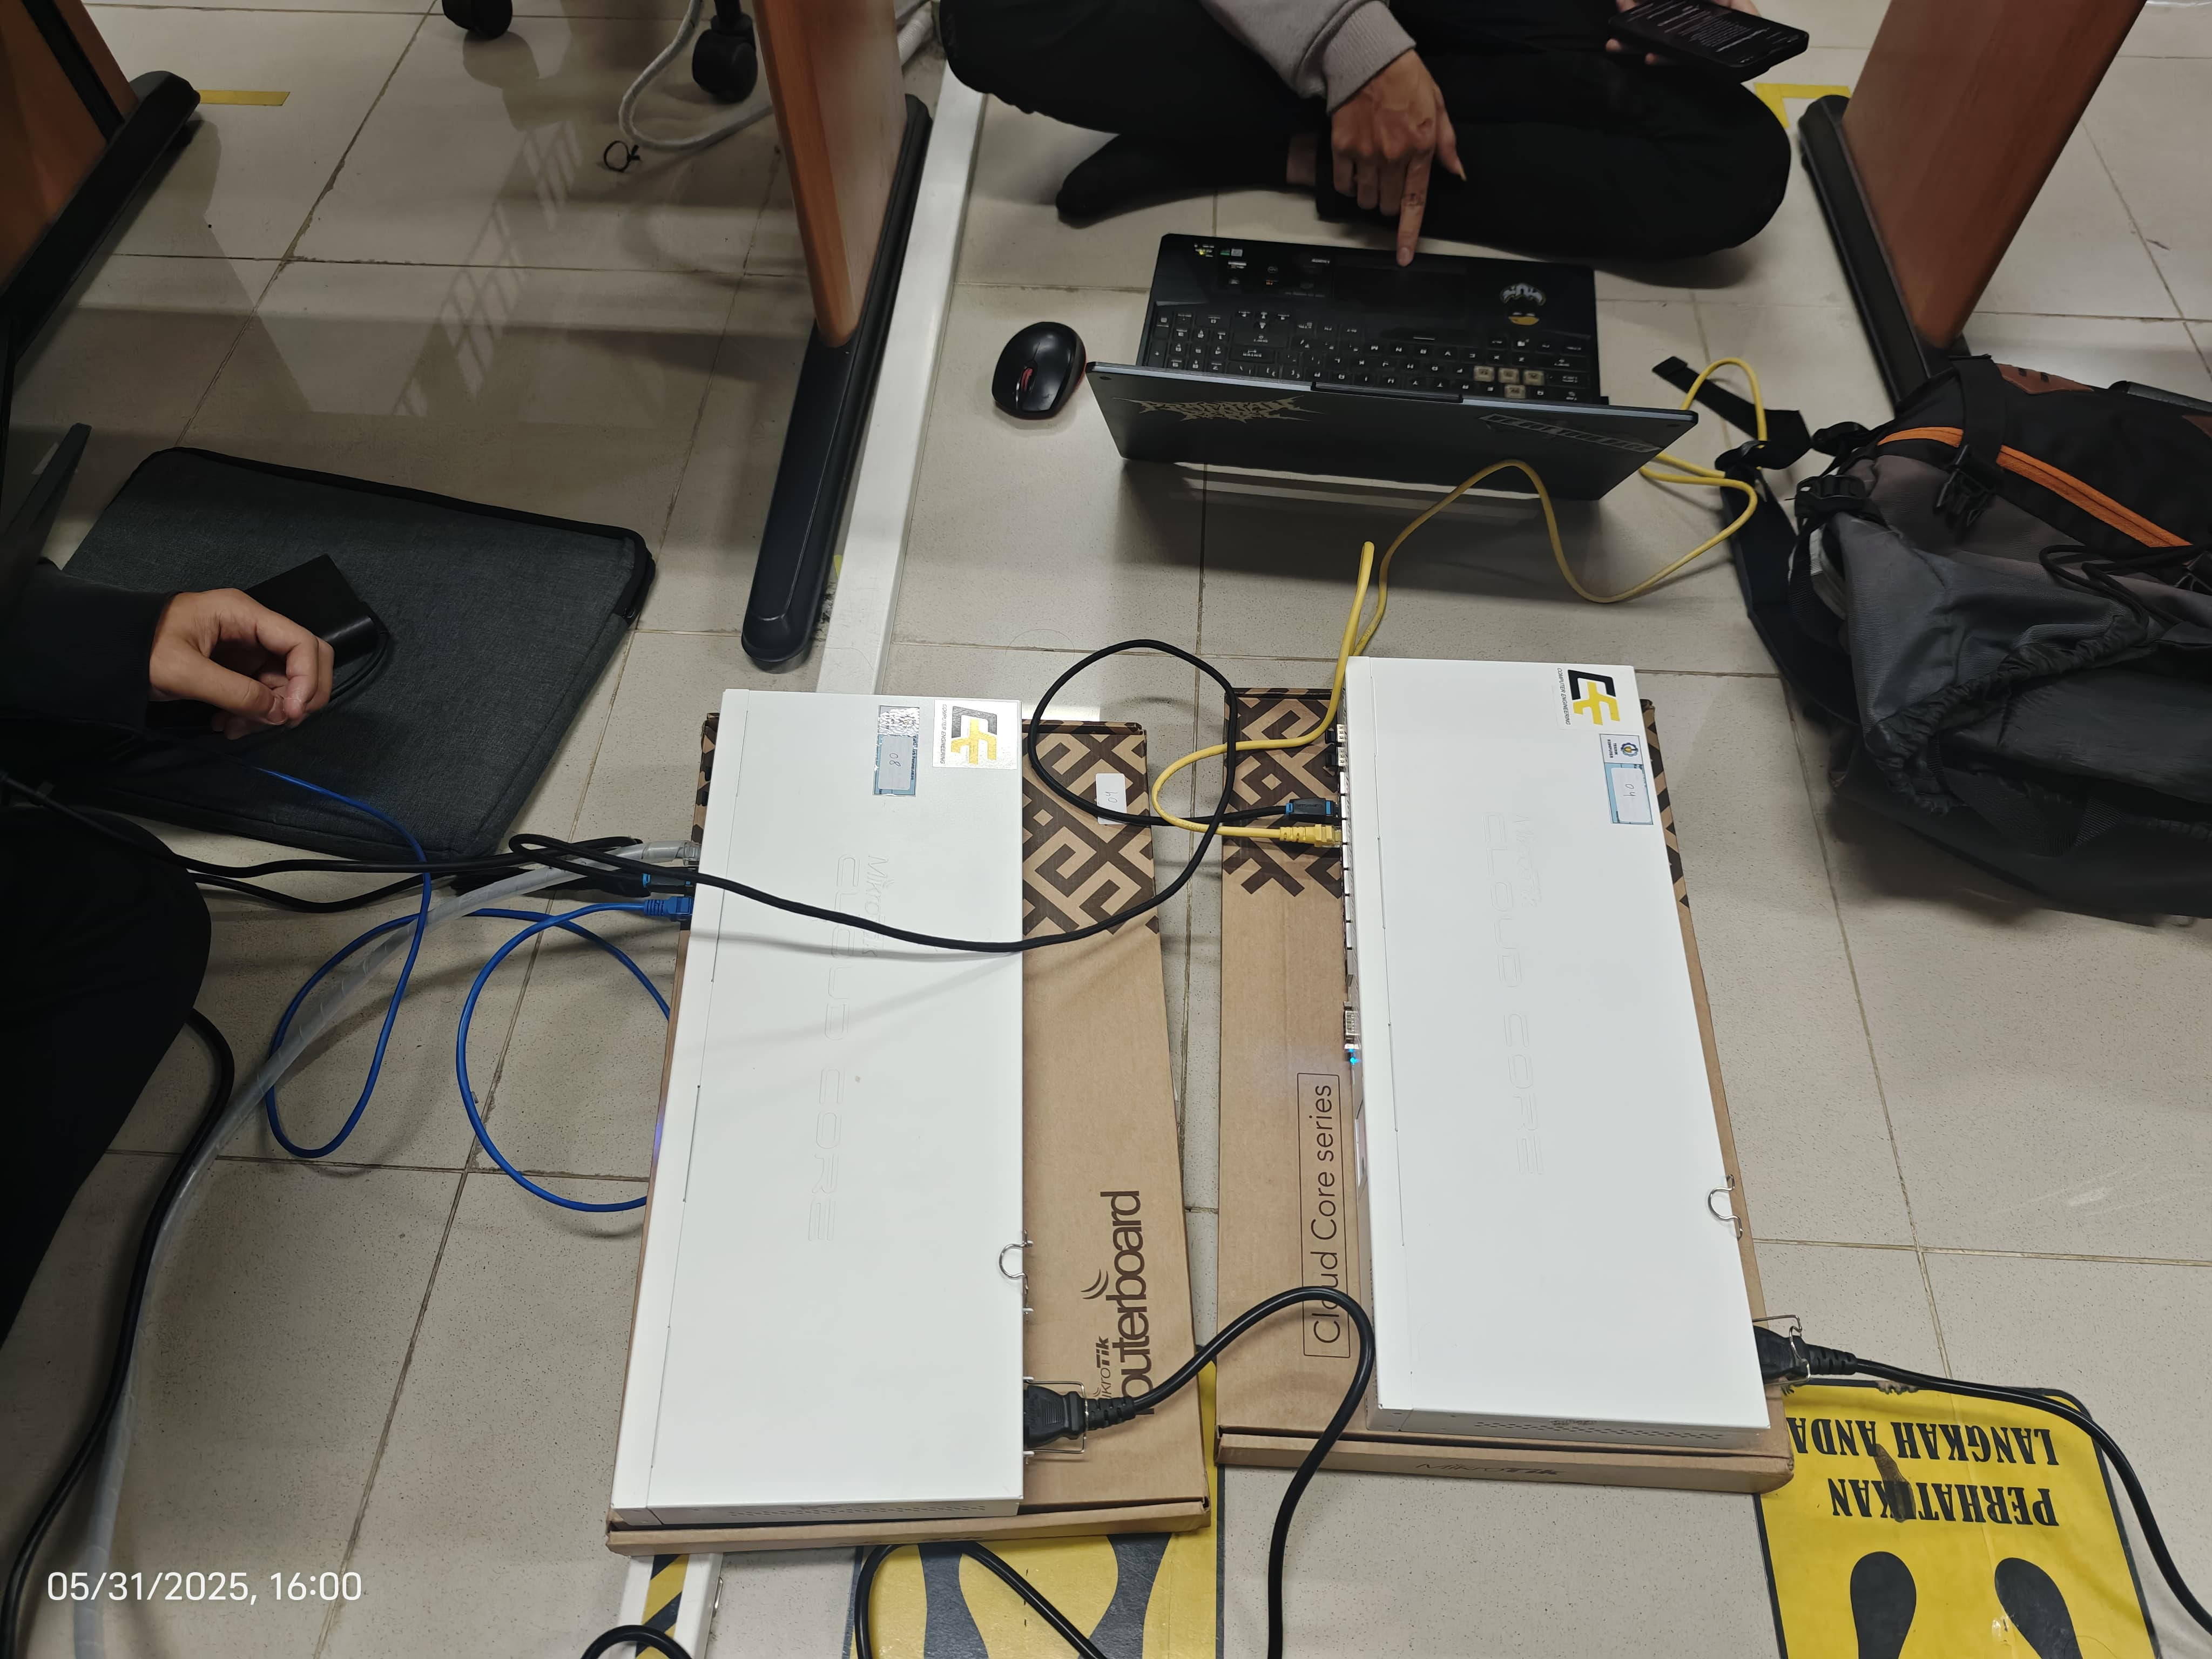
\includegraphics[width=0.7\textwidth]{img4/lampiran4.jpeg} 
    \caption{Dokumentasi praktikum.}
\end{figure}

\end{document}

\end{document}